\chapter{Analisi di Steiner}

L'introduzione dell'analisi di Downs stimolò diversi ricercatori e clinici a sviluppare le proprie analisi: quello che ne seguì fu una proliferazione di marker cefalometrici che non fecero altro che confondere i clinici. Cecil C. Steiner selezionò quelli che per lui erano i parametri più significativi, e sviluppò un'analisi che credeva potesse fornire il massimo numero di informazioni cliniche con il minor numero di misurazioni.

Vennero quindi scelte alcune misure, e furono determinate delle medie statistiche su un numero di pazienti normo-occlusi.

Nell'analisi delle teleradiografie latero-laterali, Steiner propose la valutazione separate di varie parti del cranio, nello specifico i tessuti scheletrici, i tessuti dentali e i tessuti molli. L'analisi scheletrica si propone di porre in relazione la mascella e la mandibola tra di loro e con le ossa del cranio. L'analisi dentale mette in relazione gli incisivi superiori e inferiori con le rispettive basi ossee e tra di loro. Infine, l'analisi dei tessuti molli fornisce un mezzo per valutare il bilanciamento e l'armonia del profilo facciale inferiore\footcite{Steiner1953,Steiner1959,Steiner1960}.

A tutt'oggi, questa è la tecnica più utilizzata, data la relativa semplicità e velocità d'esecuzione.

\section{Analisi scheletrica}
Nelle analisi antropologiche tradizionali, così come nell'analisi di Downs, il piano di riferimento era il \textit{piano di Francoforte}. Sulle teleradiografie latero-laterali è però spesso difficile identificare i punti Porion e Orbitale, per la determinazione di tale piano. Steiner scelse quindi la \textbf{base cranica anteriore} (Sella-Nasion) come piano di riferimento della sua analisi. Il vantaggio di utilizzare due punti ``mediani'' è che si muovono minimamente quando la testa devia dalla posizione di profilo, o quando la testa ruota nel cefalostato.

\begin{figure}[p!]
\subfloat[][]
   {\label{fig:steiner_sna}\fbox{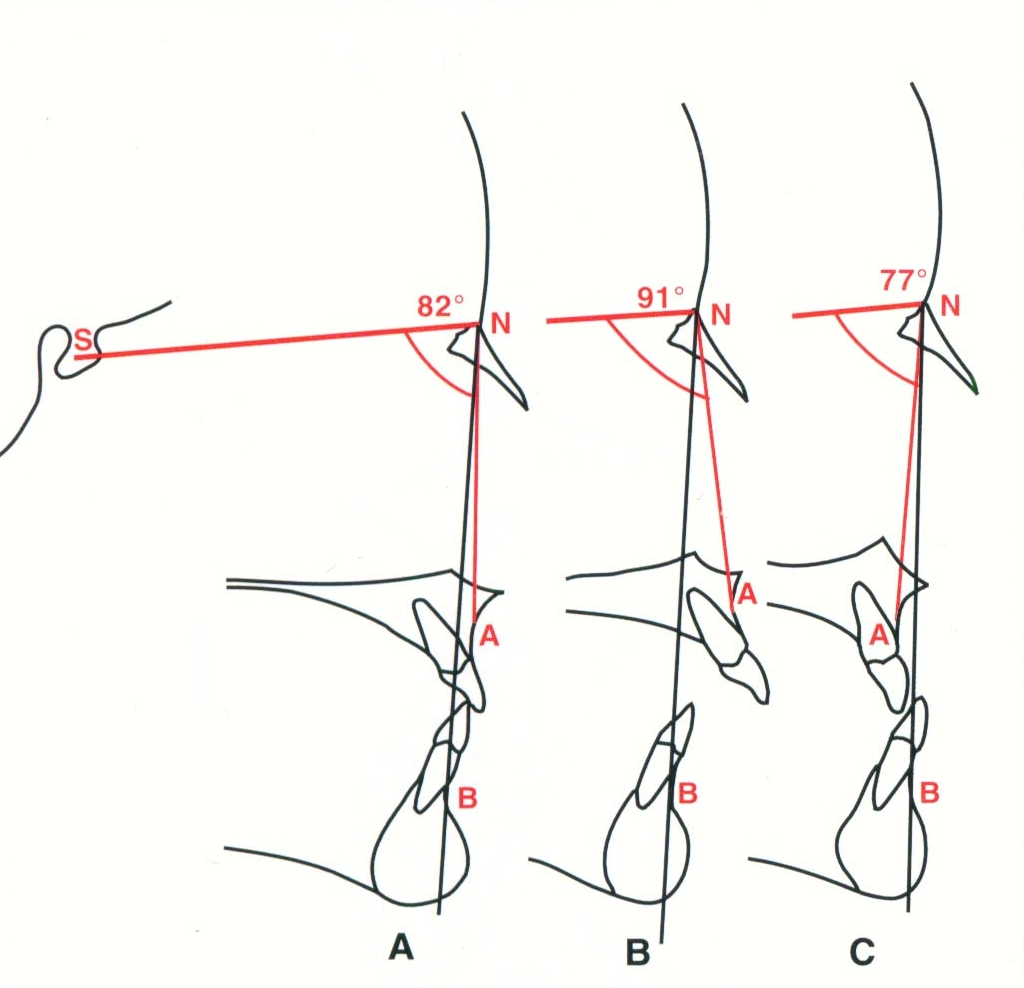
\includegraphics[width=.45\textwidth]{./images/steiner_sna.jpg}}} \quad
\subfloat[][]
   {\label{fig:steiner_snb}\fbox{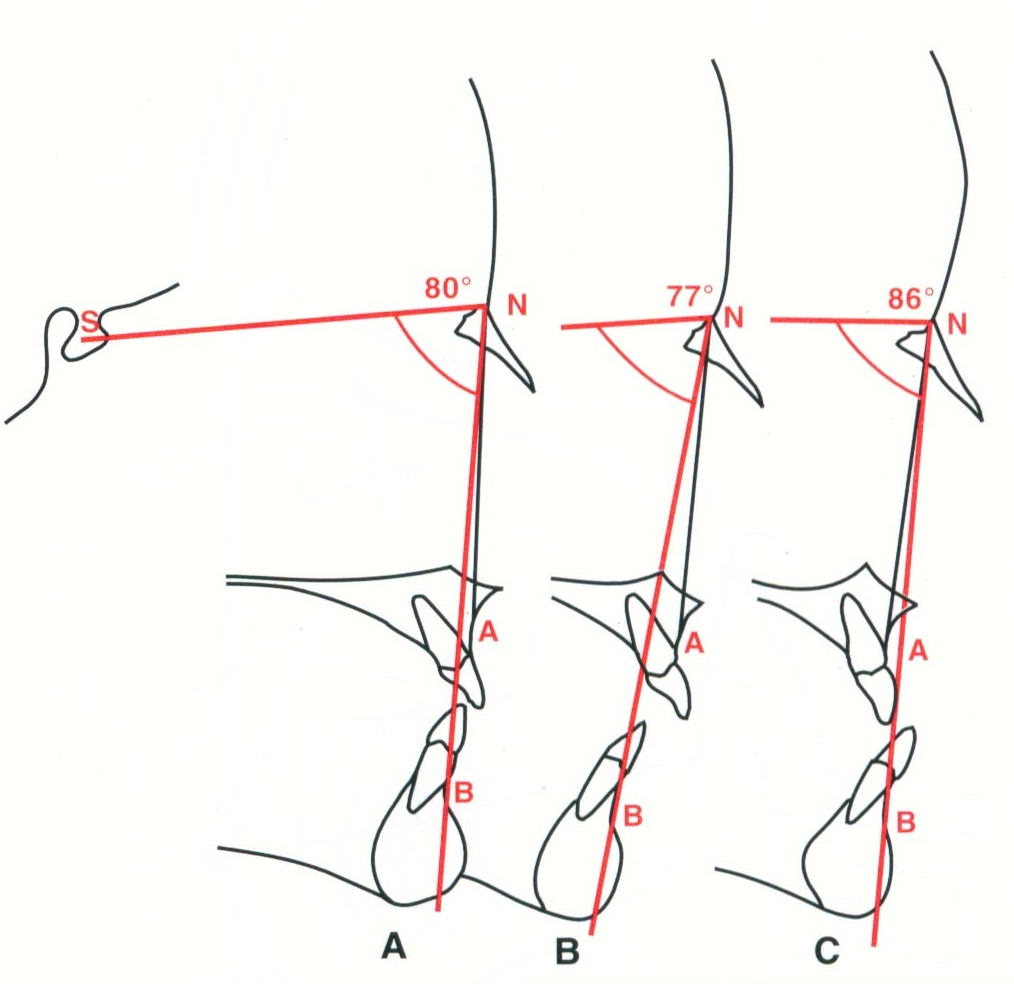
\includegraphics[width=.45\textwidth]{./images/steiner_snb.jpg}}}
 \centering
 % steiner_sna.jpg: 1024x988 pixel, 72dpi, 36.12x34.85 cm, bb=0 0 1024 988
 \caption{\subref{fig:steiner_sna} \angolo{SNA}: profilo normale, profilo retruso, profilo protruso. \subref{fig:steiner_snb} \angolo{SNB}: profilo normale, profilo retruso, profilo protruso.}
 \label{fig:steiner_sna_snb}
\end{figure}
\begin{figure}[p!]
 \centering
 \fbox{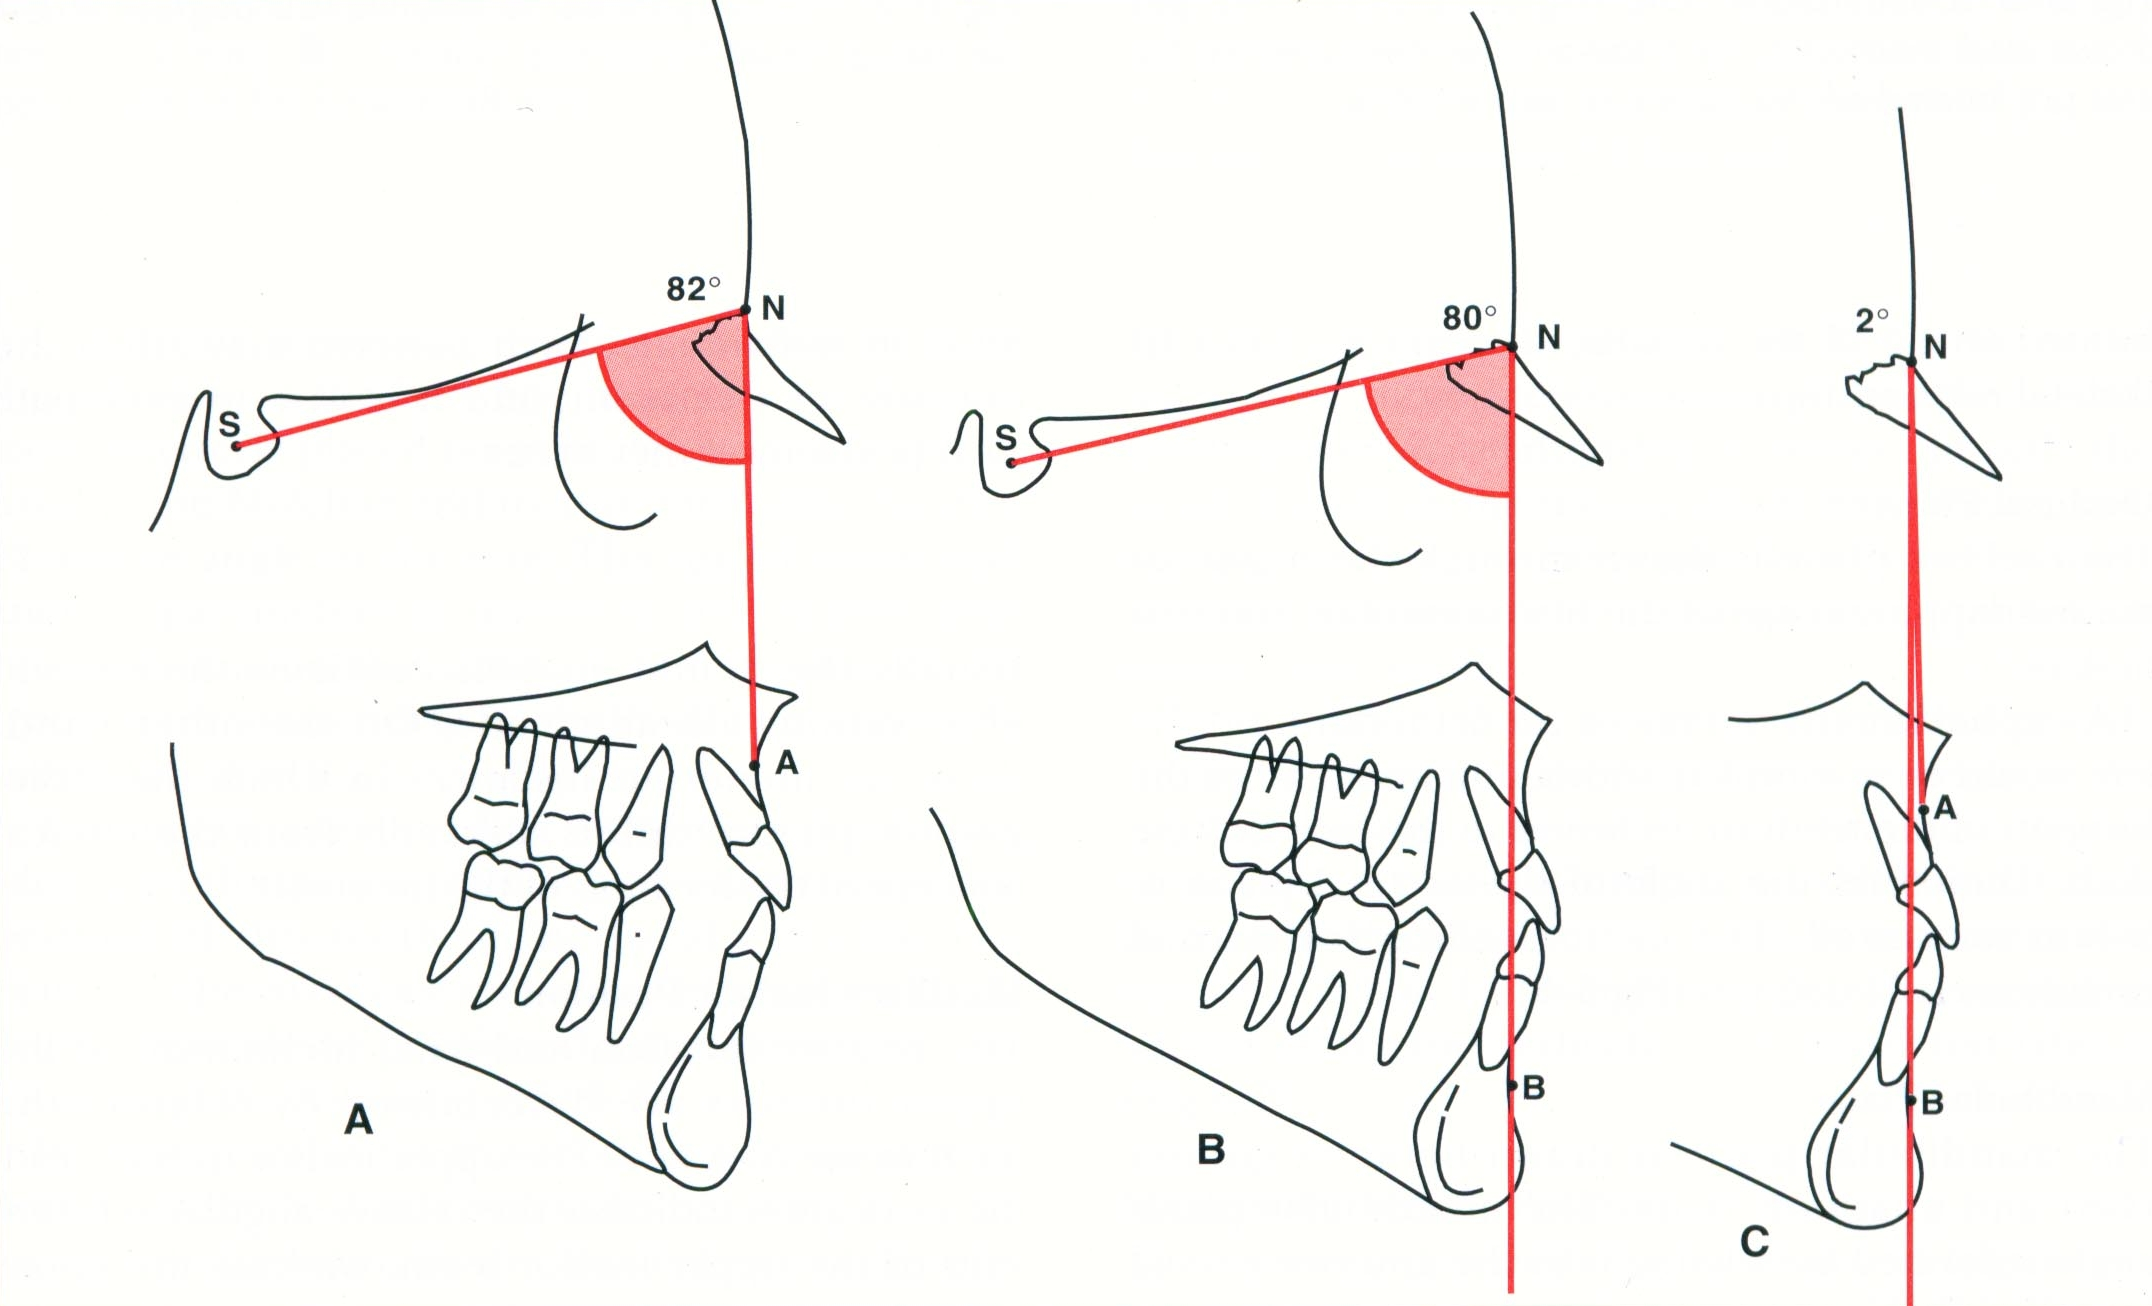
\includegraphics[width=.9\textwidth]{./images/steiner_anb.jpg}}
 % steiner_anb.jpg: 2152x1306 pixel, 72dpi, 75.92x46.07 cm, bb=0 0 2152 1306
 \caption{l'angolo interincisale \angolo{ANB} è dato dalla differenza tra \angolo{SNA} e \angolo{SNB}.}
 \label{fig:steiner_anb}
\end{figure}

\paragraph{Mascella}
I punti A e B vengono considerati come i limiti anteriori delle basi apicali rispettivamente della mascella e della mandibola. Perciò, per determinare la posizione della mascella rispetto alla base cranica, viene calcolato l'angolo \angolo{SNA}, il cui valore medio è 82° (fig. \vref{fig:steiner_sna}). Se il valore angolare è maggiore, la mascella è si trova in posizione anteriore rispetto alla base cranica. Di contro, se il valore inferiore, la mascella si troverà posizionata posteriormente.

\paragraph{Mandibola}
Per valutare la posizione della mandibola, viene calcolato l'angolo \angolo{SNB} (valore medio 80°, fig. \ref{fig:steiner_snb}). Un angolo minore indica una mandibola retrusa, un angolo maggiore indica una mandibola protrusa.

\paragraph{Relazione tra mascella e mandibola}
Valutando i valori \angolo{SNA} e \angolo{SNB}, solitamente è possibile riconoscere il segmento osseo malposizionato. Il valore più significativo è, comunque, l'angolo \angolo{ANB}, che fornisce informazioni sulla posizione dei due segmenti ossei uno relativo all'altro (fig. \vref{fig:steiner_anb}).

Steiner sosteneva come \angolo{SNA} non fosse importante quanto \angolo{SNB} e \angolo{ANB}, in quanto indica solamente una retrusione o protrusione rispetto alla base del cranio. Piuttosto, è più importante la discrepanza tra mascella e mandibola. Il valore medio dell'angolo \angolo{ANB} è di 2°: un valore maggiore indica una \textit{tendenza} alle \textit{Classe II scheletrica}, e più è grande questo valore, più difficile sarà correggere la malocclusione. Valori minori dell'angolo, e valori sotto lo zero, indicano che la mandibola è protrusa rispetto alla mascella, suggerendo una \textit{Classe III scheletrica}.

\paragraph{Piano occlusale}
Il piano occlusale viene disegnato attraverso la zona delle cuspidi sovrapposte tra i primi premolari e i primi molari. Questo piano viene utilizzato per la misura dell'angolo con il piano \punto{S}-\punto{N}. Il valore medio è di 14°.

\paragraph{Piano mandibolare}
Il piano mandibolare viene disegnato tra gonion (\punto{Go}) e gnathion (\punto{Gn}). L'angolo del piano mandibolare, che si forma tra questo e il piano \punto{S}-\punto{N}, ha un valore medio di 32°. Valori eccessivamente elevati o ridotti suggeriscono un modello di crescita rispettivamente iper- o ipodivergente. Questo modello di crescita può influenzare la riuscita del trattamento, ed è quindi saggio anticipare tali problemi.

\begin{wrapfigure}{R}{.4\textwidth}
 \centering
 \fbox{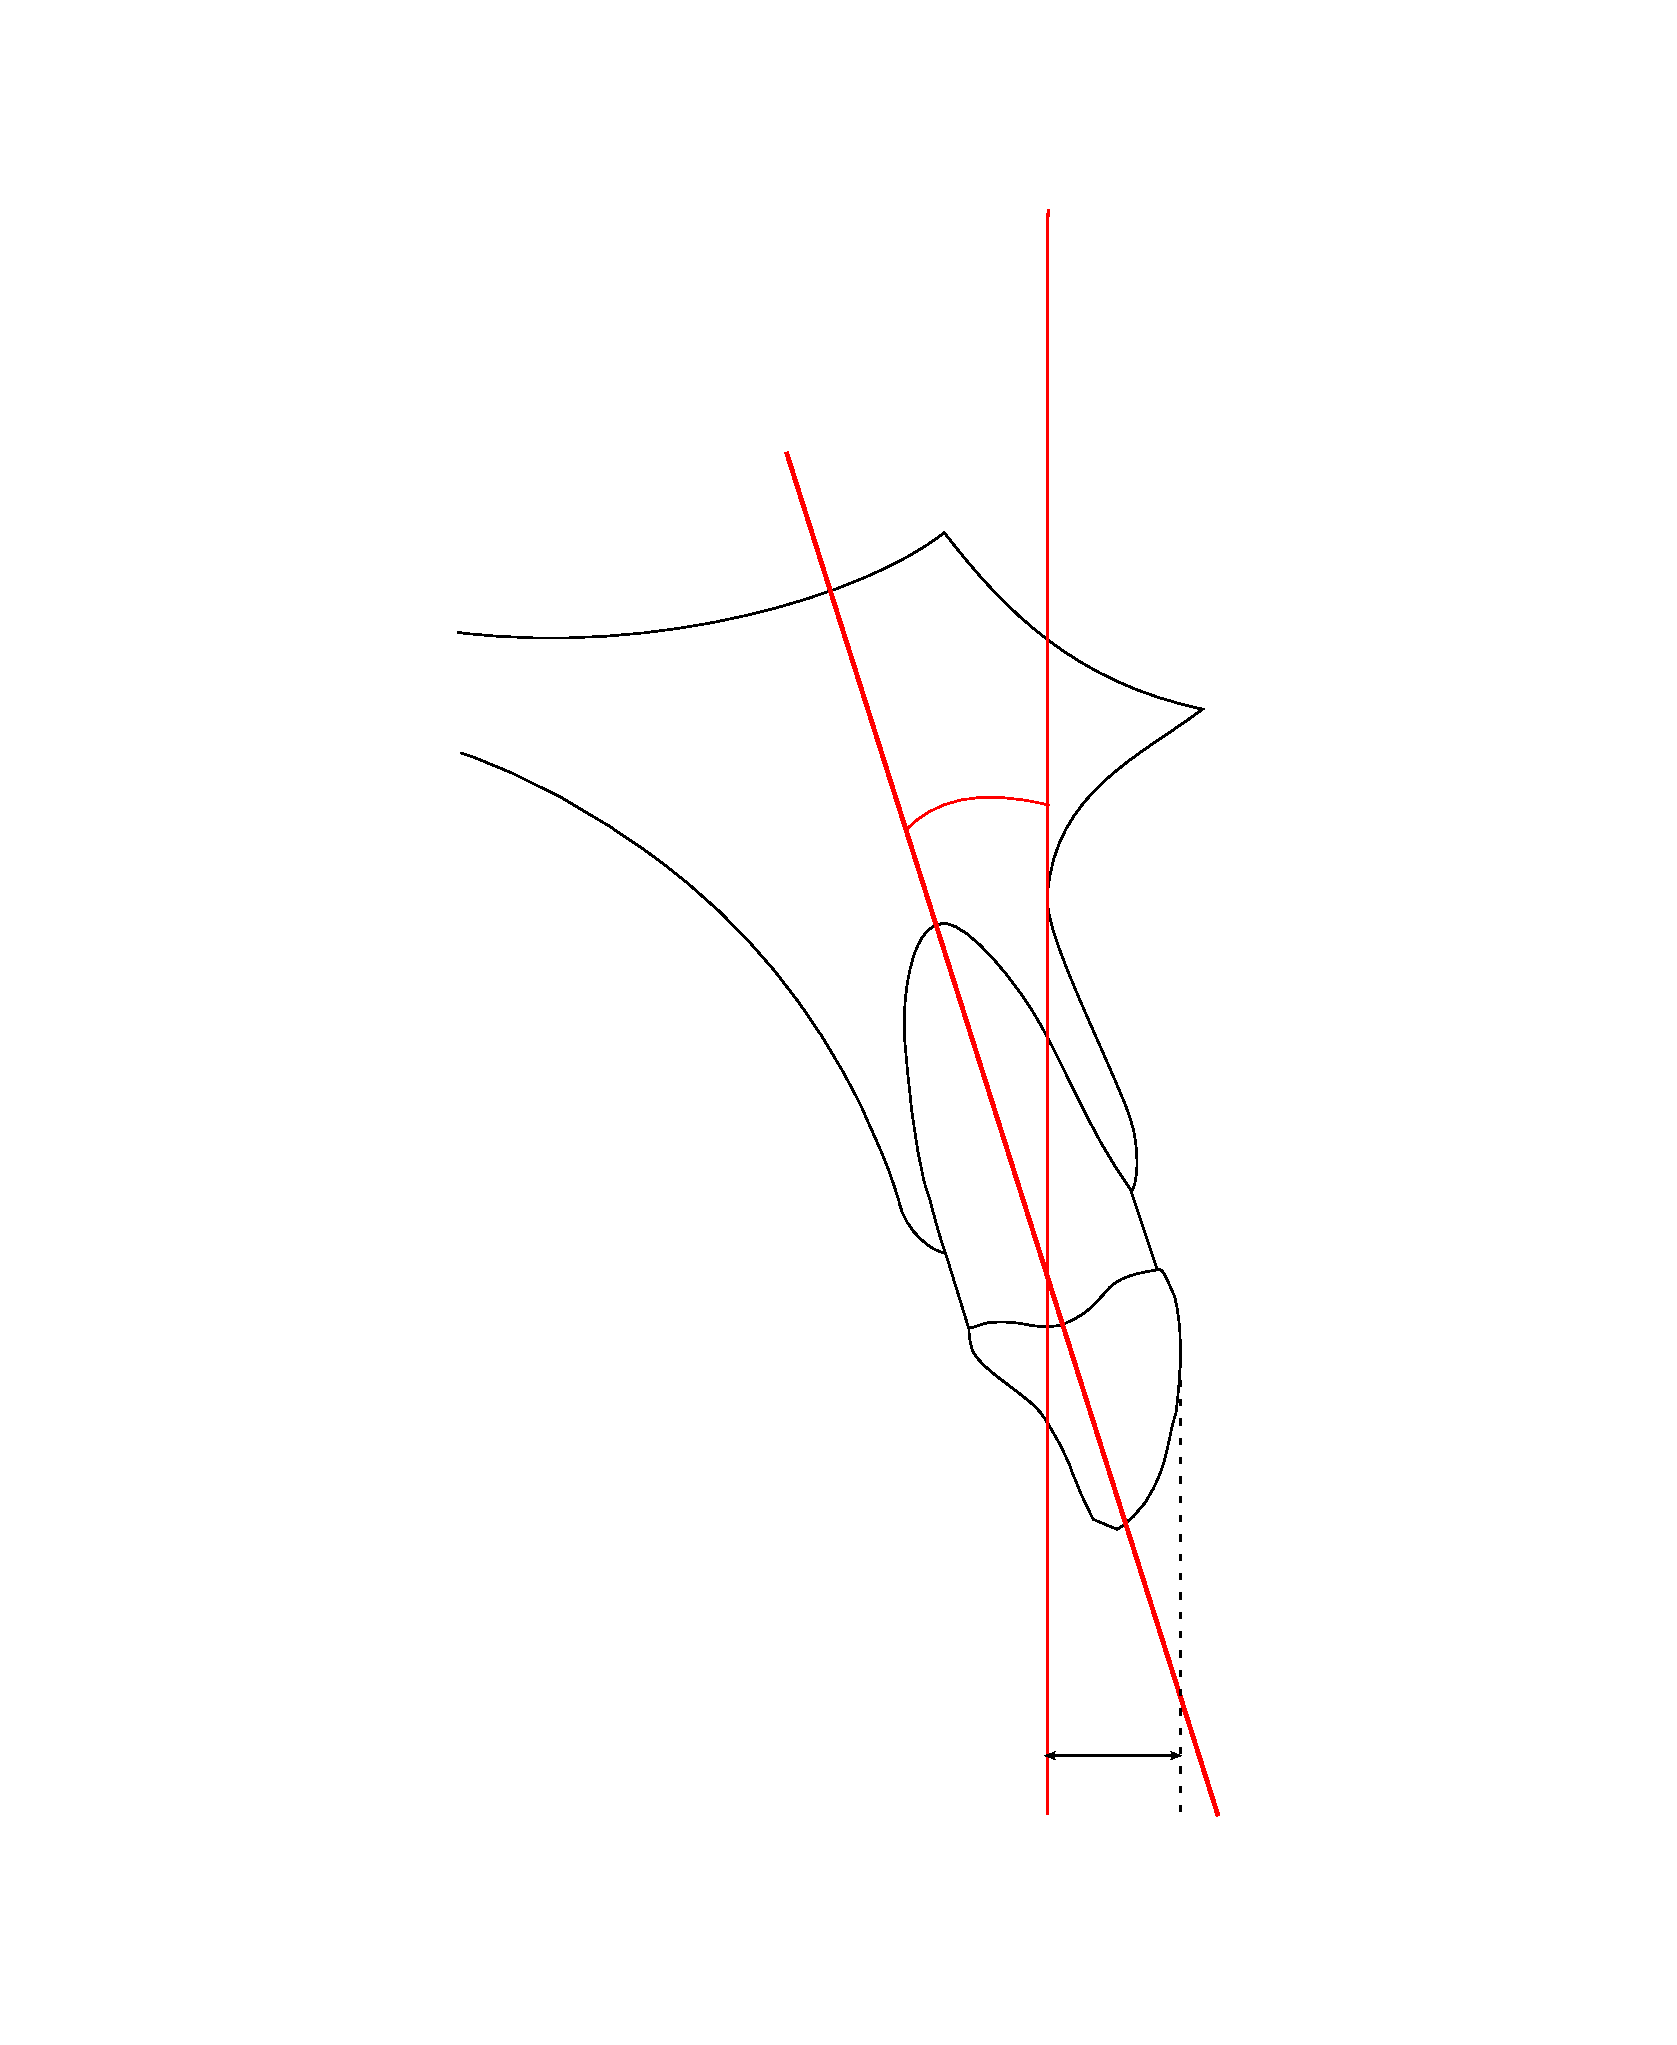
\includegraphics[width=.4\textwidth]{./images/steiner_incisale.pdf}}
 % steiner_incisale.jpg: 1006x1227 pixel, 72dpi, 35.49x43.29 cm, bb=0 0 1006 1227
 \caption{Posizione e angolazione ``ideale'' dell'incisivo superiore secondo Steiner}
 \label{fig:steiner_incisivo_superiore}
\end{wrapfigure}

\section{Analisi dentale}
Solitamente l'analisi dentale serve a confermare le valutazioni cliniche già compiute. D'altro canto, esistono numerosi casi in cui le valutazioni radiografiche differiscono notevolmente da quelle cliniche.

\paragraph{Posizione incisivo superiore}
La posizione degli incisivi superiori viene determinata correlando i denti alla linea \punto{N}-\punto{A}. È possibile considerare due valori: il primo riguarda l'angolazione dell'asse del dente e viene calcolato misurando il valore in gradi dell'angolo tra \punto{N}-\punto{A} e l'asse del dente. Il secondo valuta il posizionamento relativo, misurato in millimetri tra \punto{N}-\punto{A} e il margine incisale.

Usando questo metodo, gli incisivi centrali superiori dovrebbero essere posizionati in modo tale da avere il margine incisale ad una distanza di 4mm dalla linea, e un'inclinazione di 22°.

La sola valutazione dell'angolazione dell'incisivo superiore non è infatti sufficiente a dare un giudizio sulla posizione dei denti: potrebbe infatti capitare che l'angolazione sia corretta, ma che il dente sia traslato in avanti o indietro rispetto alla linea \punto{N}-\punto{A} (fig. \ref{fig:steiner_traslazione}).

Allo stesso modo, la sola rilevazione della distanza millimetrica del margine incisale non è sufficiente. Non è difficile immaginare un incisivo a 4mm di distanza, ma inclinato diversamente (fig. \ref{fig:steiner_rotazione}).

\begin{figure}[p!]
\subfloat[][]
   {\label{fig:steiner_traslazione}\fbox{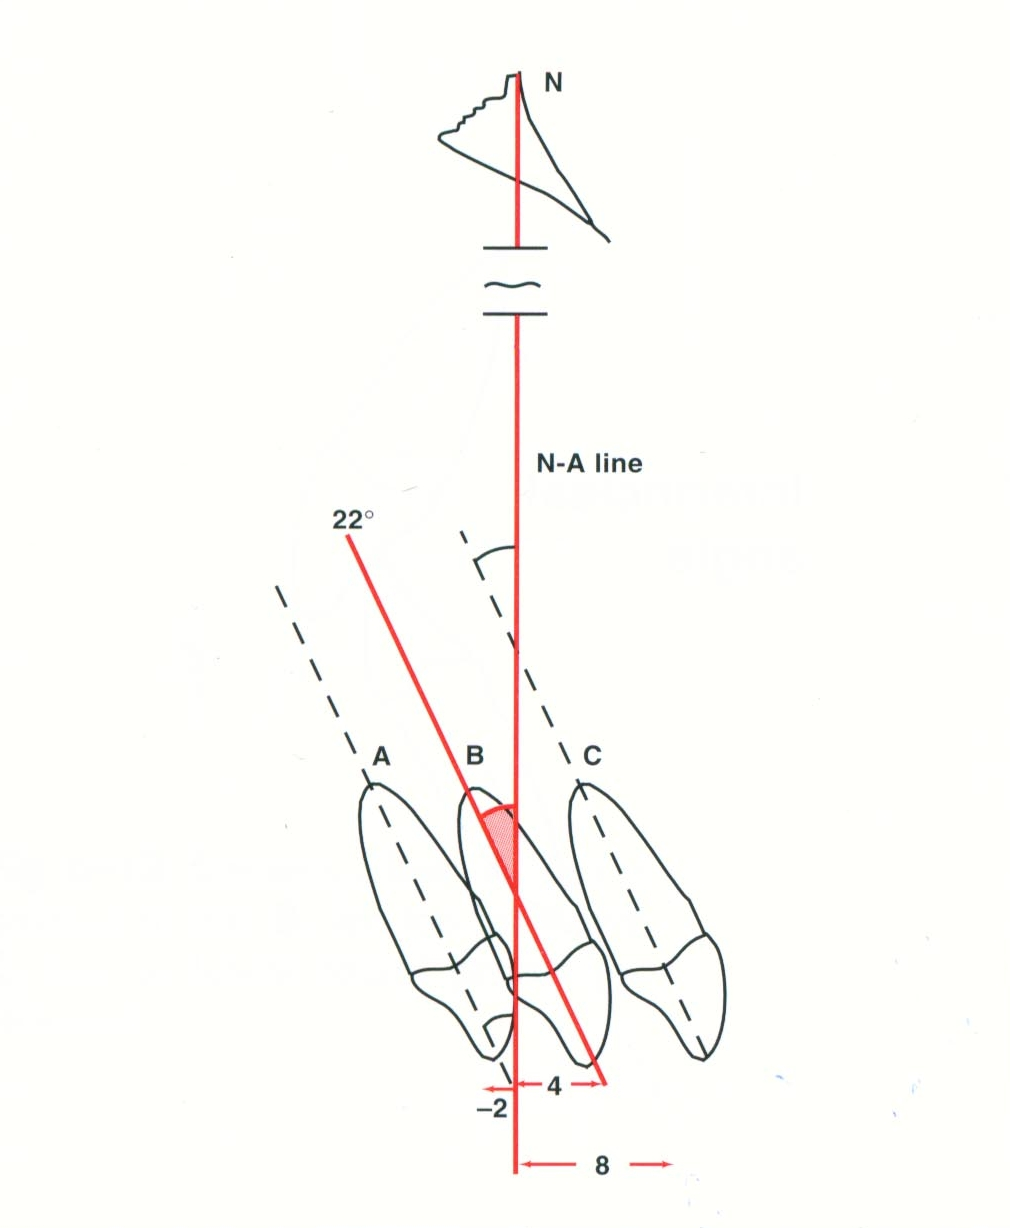
\includegraphics[width=.45\textwidth]{./images/steiner_incisivo_traslazione.jpg}}} \quad
\subfloat[][]
   {\label{fig:steiner_rotazione}\fbox{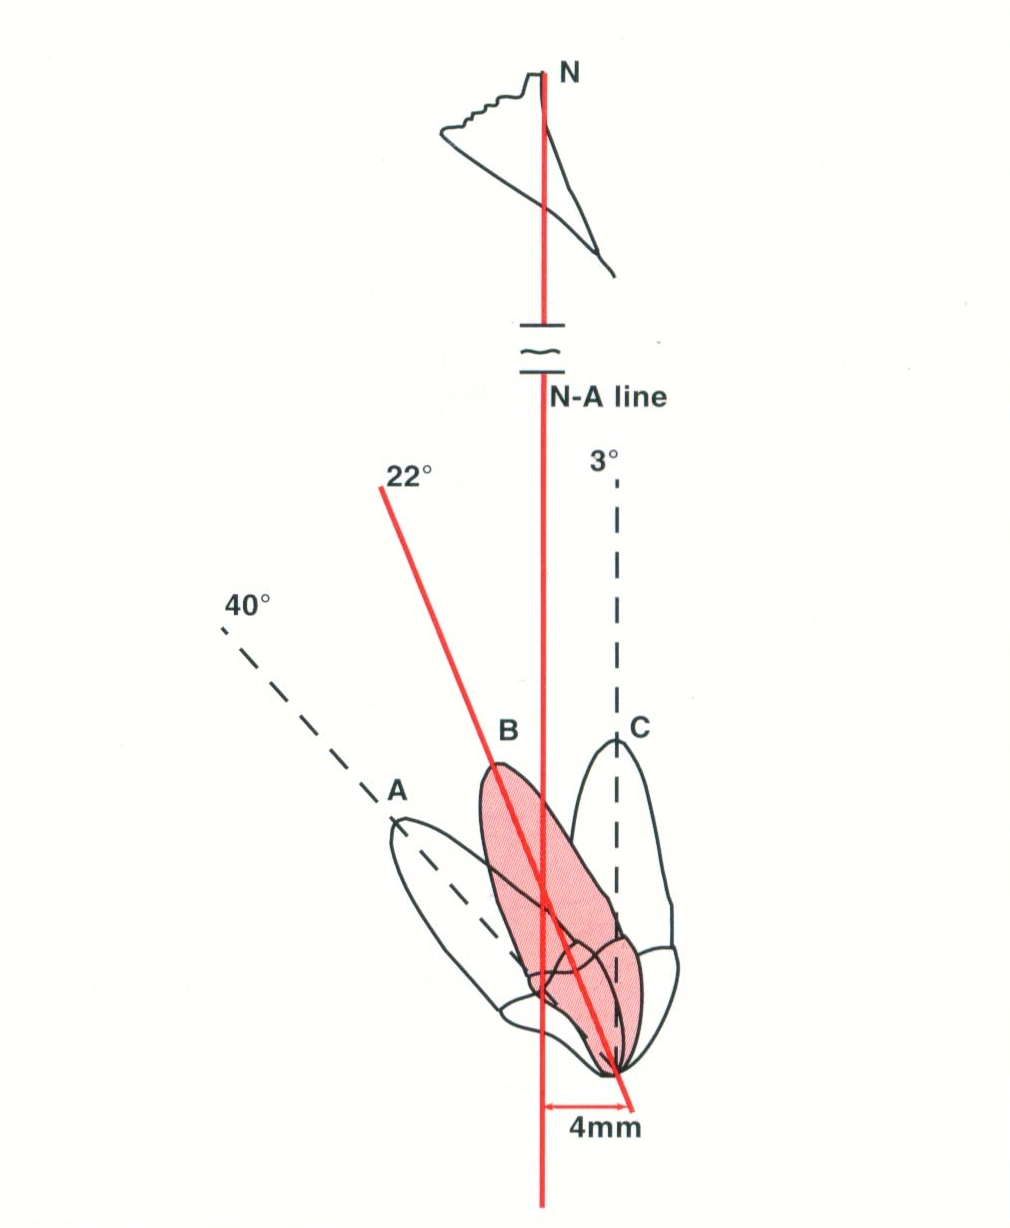
\includegraphics[width=.45\textwidth]{./images/steiner_incisivo_rotazione.jpg}}}
 \centering
 % steiner_sna.jpg: 1024x988 pixel, 72dpi, 36.12x34.85 cm, bb=0 0 1024 988
 \caption{Inclinazione e posizione dell'incisivo superiore, in relazione alla linea \punto{N}-\punto{A}: \subref{fig:steiner_traslazione} inclinazione corretta, ma posizione variabile; \subref{fig:steiner_rotazione} posizione corretta, ma inclinazione variabile.}
 \label{fig:steiner_incisivo_rototraslazione}
\end{figure}

\paragraph{Posizione incisivo inferiore}
Allo stesso modo che per l'incisivo superiore, per valutare la posizione dell'incisivo inferiore si misurano la distanza millimetrica tra margine incisale e linea \punto{N}-\punto{A}, e valore angolare tra questa e asse maggiore del dente.

\begin{figure}[p!]
\centering
\begin{minipage}{.44\textwidth}
 \centering
 \fbox{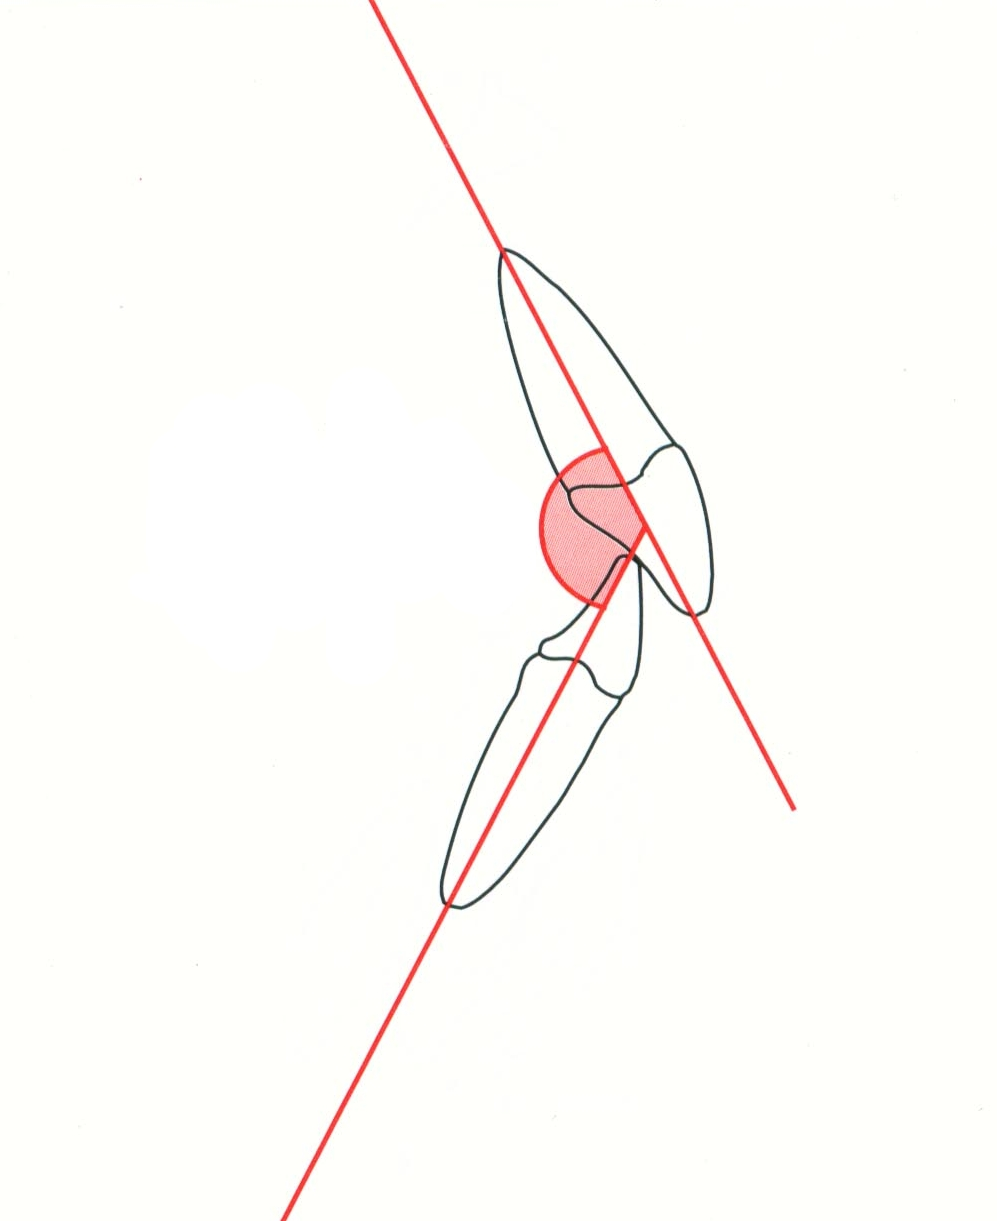
\includegraphics[width=.95\textwidth]{./images/steiner_interincisale.jpg}}
 \caption{Angolo interincisale \angolo{ANB}}
 \label{fig:steiner_interincisale}
\end{minipage}\quad\quad
\begin{minipage}{.44\textwidth}
 \centering
 \fbox{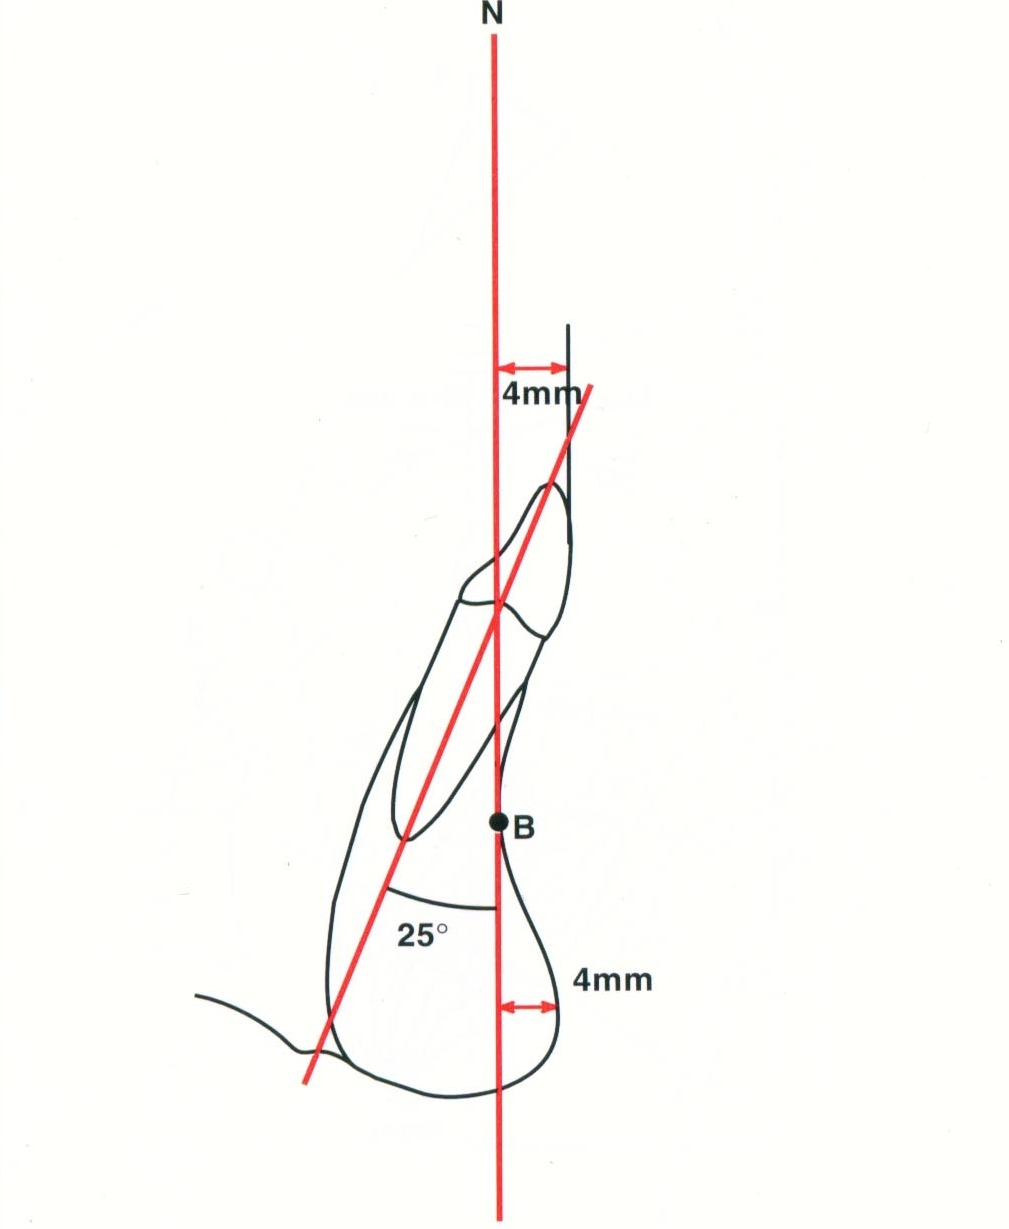
\includegraphics[width=.95\textwidth]{./images/steiner_incisivo_inferiore.jpg}}
 \caption{Rapporto tra incisivo inferiore, linea \punto{N}-\punto{A} e mento.}
 \label{fig:steiner_incisivo_inferiore}
\end{minipage}
\end{figure}

\paragraph{Angolo interincisale}
L'angolo interincisale (fig. \vref{fig:steiner_interincisale}) mette in relazione la posizione degli incisivi centrali superiore e inferiore. Il valore medio è 130°: valori minori o maggiori indicano una necessità di variazione dell'inclinazione di uno o entrambi gli incisivi.

\paragraph{Distanza tra \punto{N}-\punto{A} e il mento}
Visto il generoso contributo del mento al profilo facciale, è necessario tenerlo in considerazione nella valutazione cefalometrica. Il grado di prominenza del mento contribuisce al posizionamento dei denti in arcata. Idealmente, secondo Holdaway\footnote{citazione? p. 91}, la distanza tra la linea \punto{N}-\punto{A} e il mento dovrebbe essere uguale alla distanza tra la stessa linea e il margine incisale dell'incisivo inferiore (fig. \vref{fig:steiner_incisivo_inferiore}). Una discrepanza di 2mm tra questi valori è accettabile, 3mm è meno desiderabile, ma ancora tollerabile. Una discrepanza superiore ai 4mm, invece, richiede generalmente un intervento.

\section{Analisi dei tessuti molli}
L'analisi dei tessuti molli consiste in una registrazione grafica delle osservazioni cliniche effettuate durante l'esame del paziente. Essa include una valutazione dell'adattamento dei tessuti al profilo osseo sottostante, tenendo in considerazione dimensioni, forma e postura delle labbra. Viene inoltre analizzato lo spessore dei tessuti molli sulla sinfisi mentoniera e sulla struttura nasale, e al loro rapporto con la parte inferiore della faccia.

\begin{figure}[h!]
 \centering
 \fbox{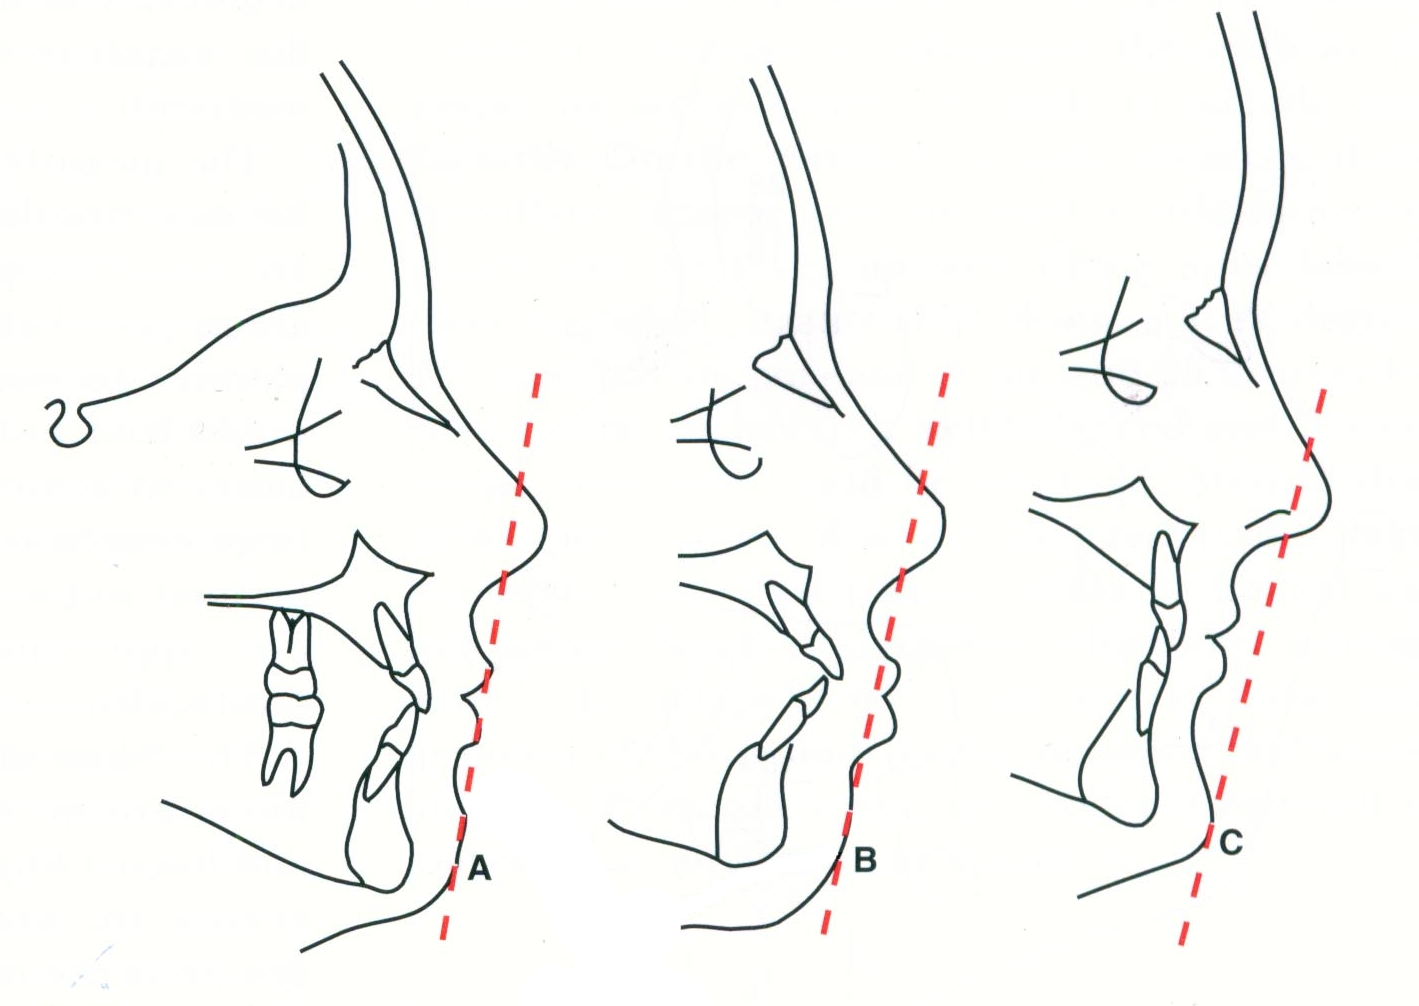
\includegraphics[width=.75\textwidth]{./images/steiner_linea_s.jpg}}
 % steiner_linea_s.jpg: 1419x1006 pixel, 72dpi, 50.06x35.49 cm, bb=0 0 1419 1006
 \caption{Linea S di Steiner: (a) labbra in equilibrio, (b) labbra protruse, (c) profilo retruso}
 \label{fig:steiner_linea_s}
\end{figure}

Steiner, Ricketts, Holdaway e Meddifield hanno sviluppato criteri e linee di riferimento per l'armonia del profilo facciale. Sebbene non possa esistere un concetto uniforme di cosa costituisca un profilo ideale, la \textit{linea S} di Steiner (fig. \ref{fig:steiner_linea_s}) è molto usata nell'ortodonzia odierna per determinare l'equilibrio dei tessuti molli facciale. Le labbra, secondo Steiner, dovrebbero toccare una linea passante dal contorno del mento al punto mediano di una S formata dal bordo inferiore del naso. Questa linea viene chiamata \textit{linea S}.

Labbra posizionate oltre questa linea tendono alla protrusione, e il trattamento richiesto solitamente prevede un retroposizionamento dentale o scheletrico. Se invece le labbra sono posizionate posteriormente, il paziente ha un profilo generalmente interpretato come ``concavo'', la cui correzione ortodontica prevede un avanzamento dei denti, causando un avanzamento delle labbra.

\nocite{Steiner1953}